\documentclass[conference]{IEEEtran}
\IEEEoverridecommandlockouts
% The preceding line is only needed to identify funding in the first footnote. If that is unneeded, please comment it out.
\usepackage[utf8]{inputenc}
\usepackage{newunicodechar}
\usepackage[english]{babel}
\usepackage{biblatex}
\addbibresource{mybibliography.bib}
\usepackage{amsmath,amssymb,amsfonts}
\usepackage{algorithmic}
\usepackage{graphicx}
\usepackage{textcomp}
\usepackage{xcolor}
\def\BibTeX{{\rm B\kern-.05em{\sc i\kern-.025em b}\kern-.08em
    T\kern-.1667em\lower.7ex\hbox{E}\kern-.125emX}}
\graphicspath{ {./images/} }
\begin{document}


\title{Open Survey of a Convolutional Neural Network -
\\CondenseNet: An Efficient DenseNet using Learned Group Convolutions.\\
{\footnotesize Submitted as part of partial fulfillment for the Fall 2020 course: ECE 62900 - Introduction to Neural Networks. Instructor: Dr. Qingxue Zhang.}
}

\author{\IEEEauthorblockN{Priyank Kalgaonkar}
\IEEEauthorblockA{\textit{Department of Electrical and Computer Engineering} \\
\textit{Purdue School of Engineering and Technology}\\
Indianapolis, Indiana 46202, USA \\
Email: pkalgaon@purdue.edu\\
Web: www.priyankkalgaonkar.com}
}

\maketitle

\begin{abstract}
With the advent of modern embedded systems and mobile devices with limited computational power, efficient convolutional neural networks are in a great demand. A Convolutional Neural Network (CNN) is a class of Deep Neural Networks (DNN), widely used in analysis of visual images captured by an image sensor, designed to extract information and convert it in to useful representations for real-time inference of the class of the object. There are a number of different CNNs that are designed to be efficiently used on mobile devices with limited computational resources. The goal of this paper is to offer a detailed review on CondenseNet, a novel architecture developed by Gao Huang, Shichen Liu, Laurens van der Maaten, with unprecedented efficiency.\\
\end{abstract}

\begin{IEEEkeywords}
Deep Neural Network, Convolutional Neural Network, Group Convolutions.
\end{IEEEkeywords}

\section{\textbf{Introduction}}
The first working Deep Neural Network (DNN) algorithm was published by Alexey Ivakhnenko and Lapa in 1967 for supervised, deep, feed-forward,
multi-layer perceptions \cite{1}. In 1971, Alexey Ivakhnenko published another paper describing a DNN with eight layers trained by multi-parametric datasets \cite{2}. Fast forwarding to the 21st century, DNN has become an important part of Computer Vision, Natural Language Processing, Speech Recognition, Social Network Filtering, to name a few. Due to the digitization of the human society, inexpensive cameras and Internet of Things (IoT), we now have a fairly large amount data which enables to train a large neural network architecture to predict/infer a number of classes of objects.

Following a graph that demonstrates how scale drives the deep learning progress. The horizontal axis of the graph plots the amount of data and the vertical axis plots the performance of the learning algorithm. Thus, it can be inferred from this graph that in order to achieve a high performance of the neural network's learning algorithm, a large neural network such as AlexNet needs to be trained on a large amount of data. However, for the Traditional Learning Algorithm such as Logistic Regression, the performance at one time flats out and no longer increases. Hence, it can be trained on a small amount of data.\\

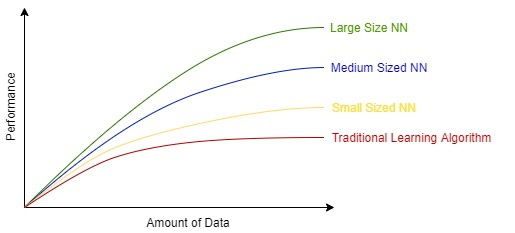
\includegraphics[scale=0.48]{graph1.jpg}\\
Figure 1: Graph that demonstrates how scale drives the deep learning process.


\section{\textbf{Evolution of Neural Networks}}

\subsection{\textbf{Logistic Regression}}
Logistic Regression is a simple form of binary classification algorithm. The input is an image and each object in the image being detected is assigned a probability between 0 and with the total sum of 1. Logistic Regression takes the input and passes it through a Sigmoid activation function that exists between 0 and 1. This Sigmoid function is responsible for classifying the input i.e. the object in the image.
\begin{center}
    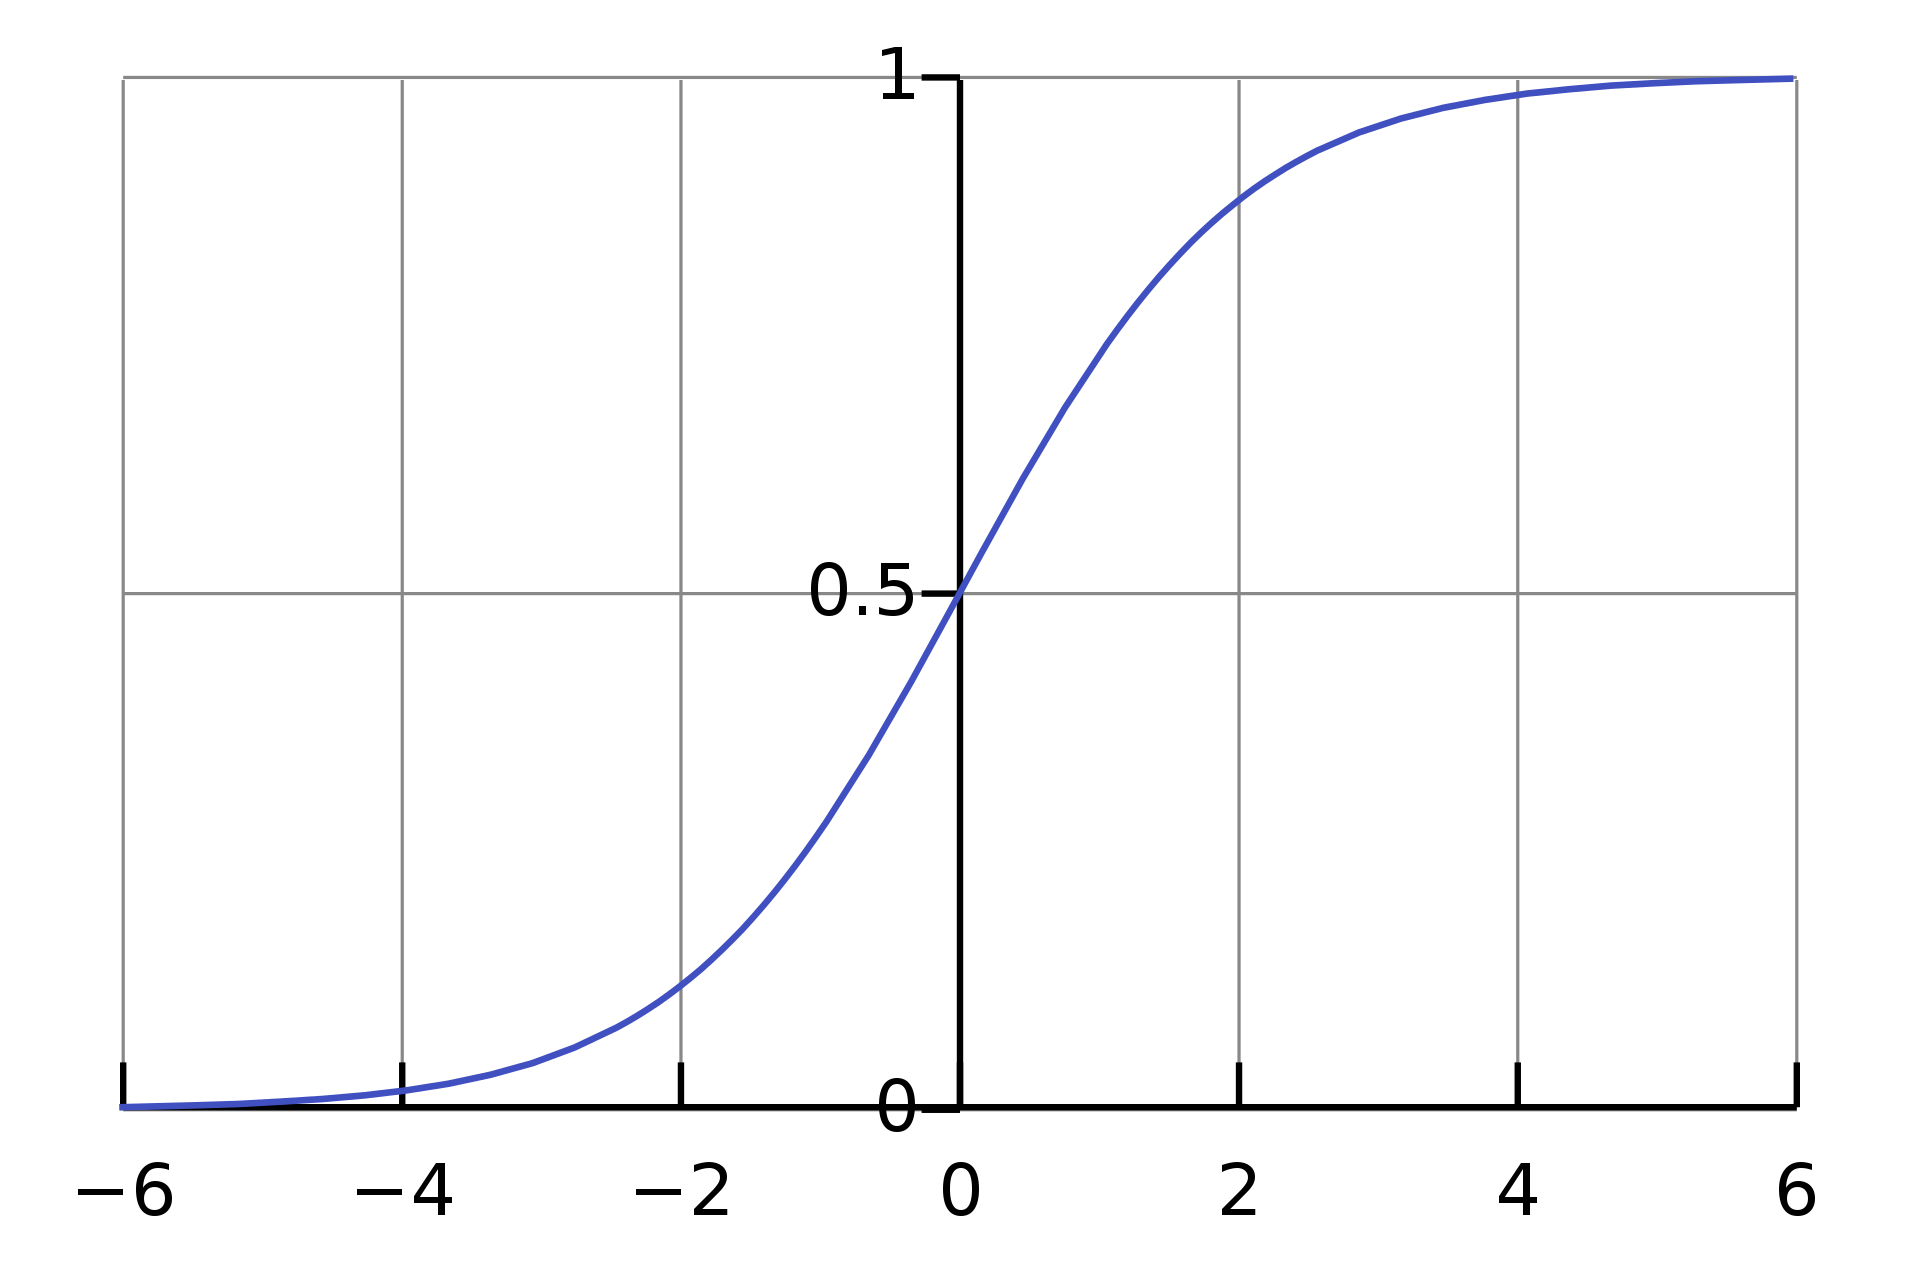
\includegraphics[scale=0.1]{1920px-Logistic-curve.svg.png}\\
\end{center}
Figure 2: Graph of Sigmoid Activation Function \cite{3}.\\

The formula for Sigmoid activation function is sig(t) =
\[\frac{1}{1+e^{-t}}\]

The Logistic Regression model takes the input as an image, for example: a 64 x 64 cat image with three channels - Red, Green and Blue, and outputs three 64 x 64 matrices. The algorithm then unrolls all these pixel values into a Feature vector $X$. The final dimension of this vector $X$ will be 64 x 64 x 3. This input is then multiplied by the Sigmoid activation function to get a value between 0 and 1 — as z increases towards positive infinity the output gets closer to $1$, and as $z$ decreases towards negative infinity the output gets closer to 0. Figure 3 below is a representation of the simple Logistic Regression Neural Network.

\begin{center}
    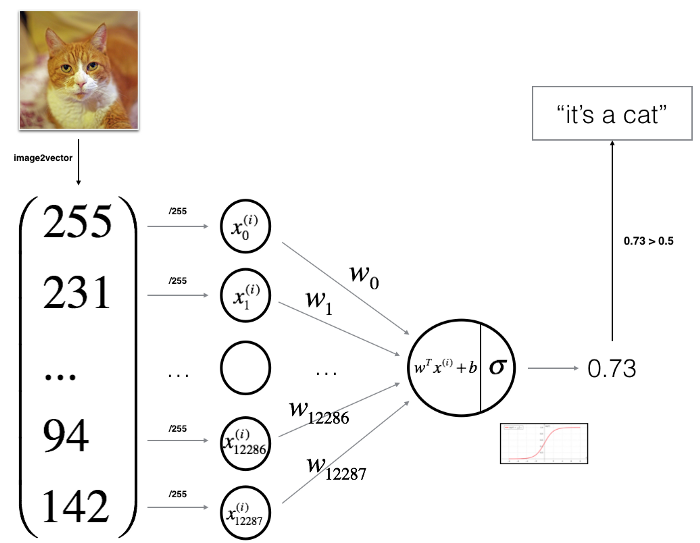
\includegraphics[scale=0.36]{LRNN.png}\\
\end{center}
Figure 3: A cat classifier that utilizes logistic regression model. \cite{7}\\

The main drawback of Logistic Regression algorithm is the assumption of linearity between the dependent and independent variables as well as the availability of structured data at all times. In the real world, the data is rarely linearly separable and always unstructured. To address these biggest pitfalls, a more complex neural networks with complicated non-linear activation functions were developed to train large amounts of data.

\subsection{\textbf{ResNet - Deep Residual Learning for Image Recognition}}
In 2015, ResNet was developed by Gao Huang, Shichen Liu, Laurens van der Maaten and Kilian Q. Weinberger to address the problem in training large (deep) neural networks. This model introduces “identity shortcut connection” that skips one or more layers, a fundamental idea behind ResNet. Instead of hoping each few stacked layers directly fit a desired underlying mapping, the authors explicitly let these layers fit a residual mapping. Formally, denoting the desired underlying mapping as $H(x)$, they let the stacked nonlinear layers fit another mapping of ${F(x) = H(x)−x}$. The original mapping is recast into $F(x)+x$. Figure 4 provides a visual representation of this novel idea.

\begin{center}
    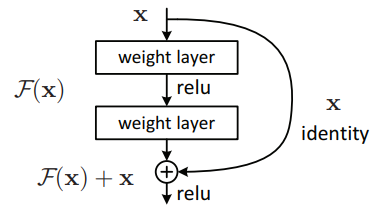
\includegraphics[scale=0.7]{ResNet.PNG}\\
\end{center}
Figure 4: Residual learning: a building block. \cite{8}\\

The authors of ResNet argue that stacking layers should not degrade the performance of the model because identity mappings can be simply stack upon the current network and the resulting architecture would perform the same/better. Although ResNet provides a revolutionary technique that forms the basis of many popular neural network architectures today, the problem of diminishing feature reuse results in weeks of training, making it's training phase very slow and expensive.

\subsection{\textbf{(Wide)ResNet - Wide Residual Networks}}
To address the issues with ResNet, in 2016, Sergey Zagoruyko and Nikos Komodakis provided a simple yet innovative technique: multiply the number of channels at each layer by a constant. For example, WideResNet-28-10 means a ResNet has a depth of 28 layers where the number of channels is 10 times bigger at each layer. The experiments performed by the author claim to have reduced computational costs and therefore, it is more interesting to have wider ResNets than excessively deep ones.

Residual block with identity mapping can be represented by the following formula:
\[x_{l+1} = x_l +F(x_l,W_l)\]
where $x_{l+1}$ and $x_l$ are input and output of the $l$-th unit in the network, $F$ is a residual function and $W_l$ are parameters of the block. Residual network consists of sequentially stacked residual blocks. \cite{9}

\begin{center}
    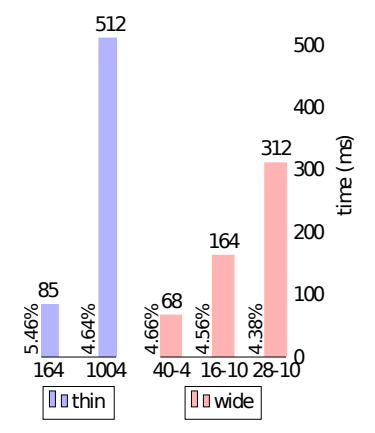
\includegraphics[scale=0.4]{WRN.PNG}\\
\end{center}
Figure 5: Time of forward+backward update per minibatch of size 32 for wide and thin networks(x-axis denotes network depth and widening factor). Numbers beside bars indicate test error on CIFAR-10, on top - time (ms). Test time is a proportional fraction of these benchmarks. Note, for instance, that wide WRN-40-4 is 8 times faster than thin ResNet1001 while having approximately the same accuracy. \cite{9}

\subsection{\textbf{DenseNet - Densely Connected Convolutional Networks}}
In 2017, Gao Huang, Zhuang Liu, Laurens van der Maaten and Kilian Q. Weinberger took the idea of residual connections even further and published a new technique which connects each layer to every other layer in a feed-forward fashion. For each layer, the feature-maps of all preceding layers are used as inputs, and its own feature-maps are used as inputs into all subsequent layers. DenseNets have several compelling advantages: they alleviate the vanishing-gradient problem, strengthen feature propagation, encourage feature reuse, and substantially reduce the number of parameters. [10] This is a very innovative technique since it facilitates the resuse of channels and neurons (tensors) that represent information at a different level of crudeness.

DenseNets introduce three new important hyperparameters, namely \cite{10}:
\begin{enumerate}
    \item \textbf{Growth Rate:} An important difference between DenseNet and other network architectures is that DenseNet can have very narrow layers, e.g., $k$ = 12. We refer to the hyperparameter $k$ as the growth rate of the network.
    \item \textbf{Bottleneck Layer:} A $1$×$1$ convolution can be introduced as bottleneck layer before each $3$×$3$ convolution to reduce the number of input feature-maps, and thus to improve computational efficiency.
    \item \textbf{Compression:} The idea of Compression is to reduce the number of channels (feature-maps) at the transition blocks. If a dense block contains $m$ feature-maps, we let the following transition layer generate $[\theta m]$ output featuremaps, where $0 <\theta \leq1$ is referred to as the compression factor. When $\theta = 1$, the number of feature-maps across transition layers remains unchanged.
\end{enumerate}

\begin{center}
    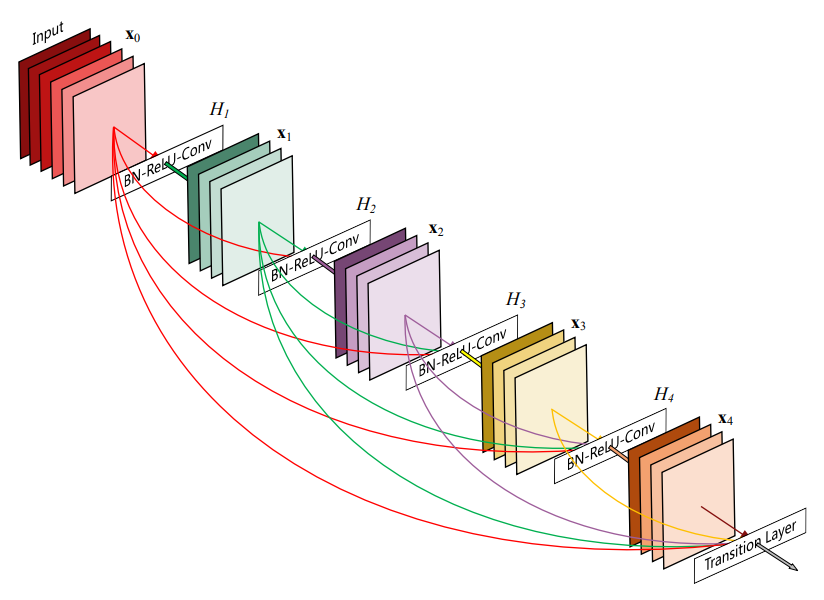
\includegraphics[scale=0.32]{DenseNEt.PNG}\\
\end{center}
Figure 6: An illustration of DenseNet. A 5-layer dense block with a growth rate of $k = 4$. Each layer takes all preceding feature-maps as input. \cite{10}

\subsection{\textbf{CondenseNet - An Efficient DenseNet using Learned Group Convolutions}}

With the development in the area of Autonomous Vehicles, Robotics and Unmanned Ariel Vehicles such as drones, a desire for highly efficient yet accurate inferring DNN models has increased. To address this demand, in 2018, Gao Huang, Shichen Liu, Laurens van der Maaten and Kilian Q. Weinberger developed CondenseNet, an improvement over DenseNet.
The two main ideas CondenseNet uses is:
\begin{enumerate}
    \item \textbf{Grouped Convolutions:} Group Convolution technique was first introduced in AlexNet in 2012 and was designed by Alex Krizhevsky, and published with Ilya Sutskever and Alex Krizhevsky's doctoral advisor Geoffrey Hinton \cite{11}. Group Convolutions helped trained AlexNet on computing machines with less powerful GPUs and limited RAM constraints at the time. The idea is to separate filters into different groups. Each group is then responsible for traditional 2D convolutions.
    \item \textbf{Connections Pruning:} The main idea of Connections Pruning technique is to enable the mapping between channels and groups to be learned by the DNN model. These approaches are effective because deep networks often have a substantial number of redundant weights that can be pruned or quantized without sacrificing (and sometimes even improving) accuracy. \cite{12}
\end{enumerate}

\begin{center}
    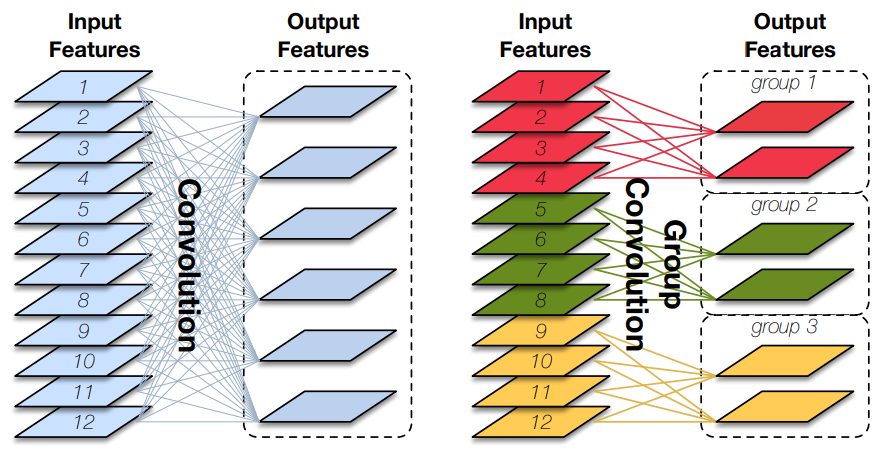
\includegraphics[scale=0.3]{CondenseNet.PNG}\\
\end{center}
Figure 7: Standard convolution (left) and group convolution (right). The latter enforces a sparsity pattern by partitioning the inputs (and outputs) into disjoint groups. \cite{12}

Group Convolutions is a unique case of sparsely connected convolutions depicted in figure 7 above. Hyper-parameter $G$ denotes number of groups in Grouped Convolutions and $C$ is the condensation factor. Thus, each convolutional group can utilize \( \frac{1}{C} \) of the input channels. Standard convolutional layers (left illustration in Figure 7) generate $O$ output features by applying a convolutional filter (one per output) over all $R$ input features, leading to a computational cost of $R×O$. In comparison, group convolution (right illustration) reduces this computational cost by partitioning the input features into G mutually exclusive groups, each producing its own outputs—
reducing the computational cost by a factor $G$ to \( \frac{RxO}{G} \). \cite{12}

\begin{center}
    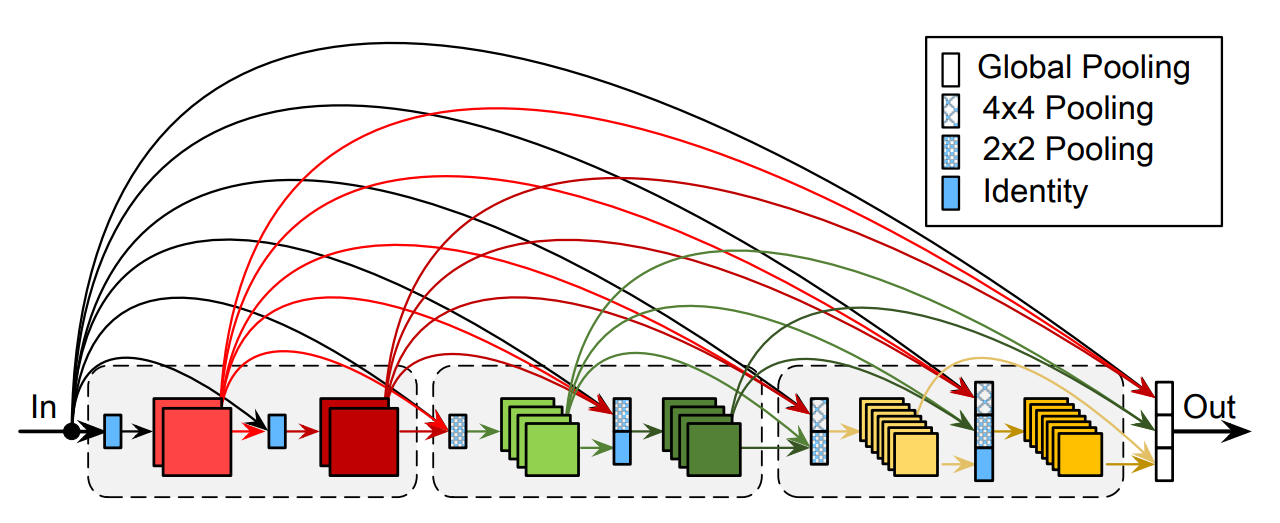
\includegraphics[scale=0.25]{CondenseNet2.PNG}\\
\end{center}
Figure 8: General representation of CondenseNet architecture. \cite{12}\\

The proposed DenseNet variant. It differs from the original DenseNet in two ways:
\begin{enumerate}
    \item layers with different resolution feature maps are also directly connected;
    \item the growth rate doubles whenever the feature map size shrinks (far more features are generated in the third, yellow, dense block than in the first).
\end{enumerate}

However, the drawback of CondenseNet CNN is that is suffers memory allocation problems like its parent model: DenseNet, which is something that can be explored by the researchers in coming years.

\section{\textbf{Conclusion}}
This paper provides a brief information about the history and evolution of Deep Neural Networks (DNN) from Linear Regression to CondenseNet with a focus on CondenseNet, an  Efficient  DenseNet  using  Learned Group  Convolutions. As desire and demand for smaller yet efficient DNN models increase with the innovations in, including but not limited to, the autonomous embedded systems with limited computing resources, the scope in this field is limitless.

\begin{thebibliography}{99}

\bibitem{1} Ivakhnenko, A. G. and Lapa, V. G. (1967). Cybernetics and forecasting techniques, pp. 5--20.
\bibitem{2} Ivakhnenko, A. G. (1971). Polynomial theory of complex systems. IEEE transactions on Systems, Man, and Cybernetics, (4), 364-378.
\bibitem{3} Wikipedia contributors. (2020, August 10). Sigmoid function. In Wikipedia, The Free Encyclopedia. Retrieved 17:38, August 31, 2020, from https://en.wikipedia.org/w/index.php?title=Sigmoidfunction
\bibitem{4} Wikipedia contributors. (2020, August 26). Gradient descent. In Wikipedia, The Free Encyclopedia. Retrieved 17:39, August 31, 2020, from https://en.wikipedia.org/w/index.php?title=Gradientdescent
\bibitem{5} Lemaréchal, C. (2012). Cauchy and the gradient method. Doc Math Extra, 251, 254.
\bibitem{6} Curry, Haskell B. (1944). "The Method of Steepest Descent for Non-linear Minimization Problems". Quart. Appl. Math. 2 (3): 258–261. doi:10.1090/qam/10667.
\bibitem{7} Index of /upsc-fever/en/data/deeplearning/images. (n.d.). Retrieved August 31, 2020, from https://upscfever.com/upsc-fever/en/data/deeplearning/images
\bibitem{8} He, K., Zhang, X., Ren, S., and Sun, J. (2016). Deep residual learning for image recognition. In Proceedings of the IEEE conference on computer vision and pattern recognition (pp. 770-778).
\bibitem{9} Zagoruyko, S., and Komodakis, N. (2016). Wide residual networks. arXiv preprint arXiv:1605.07146.
\bibitem{10} Huang, G., Liu, Z., Van Der Maaten, L., and Weinberger, K. Q. (2017). Densely connected convolutional networks. In Proceedings of the IEEE conference on computer vision and pattern recognition (pp. 4700-4708).
\bibitem{11} Krizhevsky, A., Sutskever, I., and Hinton, G. E. (2012). Imagenet classification with deep convolutional neural networks. In Advances in neural information processing systems (pp. 1097-1105).
\bibitem{12} Huang, G., Liu, S., Van der Maaten, L., and Weinberger, K. Q. (2018). Condensenet: An efficient densenet using learned group convolutions. In Proceedings of the IEEE conference on computer vision and pattern recognition (pp. 2752-2761).

\end{thebibliography}

\end{document}